\documentclass[a4paper, 10pt, oneside, titlepage]{article}
\usepackage[latin9]{inputenc}
\usepackage{unicode}
\usepackage{hyperref}
\usepackage[austrian]{babel}
\usepackage[T1]{fontenc}
\usepackage[round]{natbib}
\usepackage{graphicx}
\usepackage{supertabular}

%Anpassen der Seitenbreite
\addtolength{\hoffset}{-1.6cm}
\addtolength{\textwidth}{3.2cm}

%Anpassen der Seitenh�he
\addtolength{\voffset}{-1.2cm}
\addtolength{\textheight}{2.5cm}

%Zeilenabstand
%\linespread{1.3}

%Anpassen der Kopf- und Fu�zeilen
\usepackage{fancyhdr}
\pagestyle{fancy}
\lfoot{K�b (0250001), Theussl (0352689), Vogl (0352384), Gartner (0351427)}
\cfoot{}
\rfoot{}
\addtolength{\footskip}{2.5pt}
\renewcommand{\footrulewidth}{0.1pt}
\lhead{Leistungsbudget \textit{G-COM AG}}
\rhead{Seite \thepage}

\title{\textbf{Aufgabe 3:}\\
Erstellung eines Leistungsbudgets f\"ur die \\
\emph{G-COM AG} f\"ur 2007
}

\author{Gerold K�b (0250001)\\Stefan Theussl (0352689)\\Matthias Vogl (0352384)\\Martin Gartner (0351427)}



\begin{document}
\maketitle

%Anpassen der Paragraphenhervorhebung
\setlength{\parindent}{0pt}
\setlength{\parskip}{1.8ex plus 0.5ex minus 0.2ex}

%% INPUT-FILES

\textbf{Hinweise zur Berechnung:}

\begin{itemize}
\item Umsatzerl�se = Absatzmenge $\times$ Verkaufspreis (inkl. USt)

\item Rabatt = Bruttoerl�se (exkl. USt) $\times ~  5~ \% $

\item Skonto = Zielerl�se $\times$ 1~\%

\item Vertreterprovision = Nettoerl�se $\times$ 3~\%

\item Lohn der Produktionsabteilung = Lohnkosten je Stunde $\times$ Stunden je St\"uck $\times$ Absatzmenge

\item var. Energiekosten = Energieeinheiten je St\"uck $\times$ Absatzmenge $\times$ Energiekosten je Einheit

\item Materialeinzelkosten = Materialkosten je St\"uck $/~1.2$ $\times$ Absatzmenge

\item Frachtkosten = Fracht je St\"uck $\times$ Absatzmenge

\item sonst. var. Herstellkosten = sonst. Fertigungsgemeinkosten $\times$ Absatzmenge der Produktgruppe $/$ gesamte Absatzmenge

\item kalkulatorische Abschreibung = $68,750 + 84,000 + 50,000~=~202,750$
  \begin{itemize}
  \item Maschine 1:\\
    Wiederbeschaffungswert $/$ kalk. Nutzungsdauer = $550,000 / 8~=~68,750$
  \item Maschine 2:\\
    Restwert Anfang 2007 $\times~30~\% $ = $400,000 \times 0.7 \times 30~\%~=~84,000$
  \item Maschine 4:\\
    Keine Abschreibung wegen Ver�u�erung.
  \item neue Anlage:\\
    Keine Abschreibung, weil die Inbetriebnahme erst 2008 erfolgt.
  \item Verpackungsmaschine:\\
    Wiederbeschaffungswert $/$ kalk. Nutzungsdauer = $500,000/10~=~50,000$
  \end{itemize}

\item kalkulatorische Zinsen des Anlageverm�gens~=~BW~Maschinen~Anfang~2007~$\times~8~\%$

\item kalkulatorische Zinses des Umlaufverm�gens~=~(AB~Material~-~EB~Material)~$/~2$ = $(150,000 + 50,000) / 2 $\\
  EB = AB + Zukauf - Verbrauch = $150,000 + 180,000 / 1.2 - 250,000$~(siehe Materialeinzelkosten)~$ =~50,000$
  
\item Versicherungen (enthalten in kalk. Wagnissen) =
  2 Monate von Pr�miensumme 48,000 und 10~Monate von Pr�miensumme 54,000\\
  = $48,000 / 12 \times 2 + 54,000 / 12 \times 10 = 53,000$

\item AfA laut Finanzbuchhaltung = $120,000 + 100,000 + 50,000 = 270,000$
  \begin{itemize}
  \item Maschine 1:\\
    Anschaffungswert $/$ Nutzungsdauer = $600,000 / 5~=~120,000$
  \item Maschine 2:\\
    Anschaffungswert $/$ Nutzungsdauer = $400,000 / 4~=~100,000$
  \item Maschine 4:\\
    Keine Abschreibung wegen Ver�u�erung (Anmerkung: Normalerweise m\"usste noch die Abschreibung bis zur Ver�u�erung ber\"ucksichtigt werden. Hierzu gibt es allerdings keine Angaben!)
  \item neue Anlage:\\
    Keine Abschreibung, weil die Inbetriebnahme erst 2008 erfolgt.
  \item Verpackungsmaschine:\\
    Anschaffungswert $/$ Nutzungsdauer = $500,000/10~=~50,000$
  \end{itemize}

\item Steuer = Unternehmensergebnis $\times~25~\%$
  
\end{itemize}



\begin{figure}
\centering
\includegraphics[width = \textwidth]{bud.eps}
\end{figure}

\bibliographystyle{plainnat}
\bibliography{bibfile}


%% \appendix

\end{document}
